%-*-latex-*-
The following is a game tree:

\begin{center}
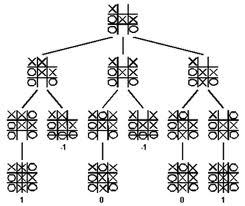
\includegraphics[width=3in]{ttt.jpg}
\end{center}

It's a tree where the nodes contain game states, describing
all the possible scenarios of a game, in this case tic-tac-toe.
The leaves are of course when there's a draw or when there's a winner.

Write a program that accepts (as command-line arguments)
an integer \verb!n!, a character \verb!c!
that is either \verb!X! or \verb!O! (that's uppercase letter and not 
zero), a
string representing an \verb!n!-by-\verb!n! tic-tac-toe
game state, print the game tree of states highlighting
the states with guaranteed wins.
Character \verb!c! represeents the player to make the next move.
You must also generate a graphviz dot file.
Details on console and dot file printout is below.
For this question, you must use the \verb!TreeNodel! class.

You may assume that the inputs are correct.
For instance if the user enters 4 for \verb!n! then the 
game state as a string has 
a length of \verb!n!$^2 = 16$.

The children for a game state is basically taking an available cell on the
game board for a player. 
The children are ordered in the usual way 
(i.e., left to right, top to bottom for available cells.)

Here's how the user will enter 
a game state. 
To enter the empty $3$-by-$3$ board,
the user enters \verb!_________!, i.e., use \verb!_! (underscore) for a space.
For this game state:
{\small
\begin{Verbatim}
       X|O|X
       -+-+-
        | |O 
       -+-+-
        | |X
\end{Verbatim}
}
the user enters \verb!XOX__O__X!.


Your printout must print the tree using
pre-order traversal of the game tree.
For each edge down the tree, indent by 4 spaces.
This printout is to the console/shell window.

Here's an input requesting for all winning moves for \verb!X!
(underlined text is user input).
Only the first few lines of output is shown.
In this case the player making the move is \verb!X!.
(Yes I know there are more \verb!X!'s than \verb!O!'s.)
\begin{console}[commandchars=\\\{\},fontsize=\small]
g++ main.cpp
\userinput{./a.out 3 X XOX__O__X}
XOX__O__X
    XOXX_O__X
        XOXXOO__X
            XOXXOOX_X (X)
            XOXXOO_XX
                XOXXOOOXX (_)
    XOX_XO__X (X)(*)
    ...
\end{console}
Next to each leaf game states, you will see \verb!(X)!
indicated that the winner is \verb!X!.
If you see \verb!(O)!, then \verb!O! is the winner.
If you see \verb!(_)!, then it's a draw.

Also, next to the children states of the root, you will see \verb!(*)!
which tells the user that that's a good move, i.e,
it's either a winning move or is guaranteed to make a winning move
in the future.
For instance the child-2 of the root is a child state
that will produce a winning move:
\begin{console}[commandchars=\\\{\},fontsize=\footnotesize]
\userinput{g++ main.cpp}
\userinput{./a.out 3 X XOX__O__X}
XOX__O__X
    ...
    XOX__OX_X (*)
    ...
\end{console}
That's because the descendents of this state looks like this:
  \begin{console}[commandchars=\\\{\},fontsize=\footnotesize]
\userinput{g++ main.cpp}
\userinput{./a.out 3 X XOX__O__X}
XOX__O__X
    ...
    XOX__OX_X (*)
        XOXO_OX_X
            XOXOXOX_X (X)
            XOXO_OXXX (X)
        XOX_OOX_X
            XOXXOOX_X (X)
            XOX_OOXXX (X)
        XOX__OXOX
            XOXX_OXOX (X)
            XOX_XOXOX (X)
    ...
\end{console}
Note that all paths lead to winning states.
Also, note that when X is making a move and there is one move that
will force a win in the future, X is still the winner.
X does not need to have all leaf nodes to be winning states.


As for the graphviz dot file, here's an example on how to label the nodes.
{\footnotesize
\begin{console}
digraph G
{
   ...
   
   XOX_X_XX_ [shape=box, fontsize=6, label="XOX\n_X_\nXX_"];
}
\end{console}
}
Obviously this should be generated by your program.

\textsc{Note.}
A game tree is essentially the intelligence
behind AI game agents.
For games even with moderate complexity,
their game trees are extremely huge.
For instance there are approximately $10^{120}$ possible game states in chess.
This is even more than the number of
atoms in the observable universe, i.e., $10^{80}$.
This means that there is absolutely \textit{no} 
way one can create the whole game tree
of chess and then play a game of chess intelligently.
